\begin{enumerate}[label=\thesubsection.\arabic*,ref=\thesubsection.\theenumi]
\item The two opposite vertices of a square are $(–1, 2)$  and $ (3, 2)$. Find the coordinates of the other two vertices.
\\
\solution
	\iffalse
\documentclass[12pt]{article}
\usepackage{graphicx}
\usepackage{amsmath}
\usepackage{mathtools}
\usepackage{gensymb}

\newcommand{\mydet}[1]{\ensuremath{\begin{vmatrix}#1\end{vmatrix}}}
\providecommand{\brak}[1]{\ensuremath{\left(#1\right)}}
\providecommand{\norm}[1]{\left\lVert#1\right\rVert}
\newcommand{\solution}{\noindent \textbf{Solution: }}
\newcommand{\myvec}[1]{\ensuremath{\begin{pmatrix}#1\end{pmatrix}}}
\let\vec\mathbf

\begin{document}
\begin{center}
\textbf\large{CHAPTER-7 \\ COORDINATE GEOMETRY}

\end{center}
\section*{Excercise 7.4}

Q4.The two opposite vertices of a square are $(–1, 2) \text{ and } (3, 2)$. Find the coordinates of the other two vertices.\\
\fi
\solution
Let
\begin{align}
\vec{A} = \myvec
{
-1 \\
 2\\
},
\vec{C} = 
\myvec
{
3\\
2\\
}
\end{align}

\begin{figure}[!h]
	\begin{center} 
	    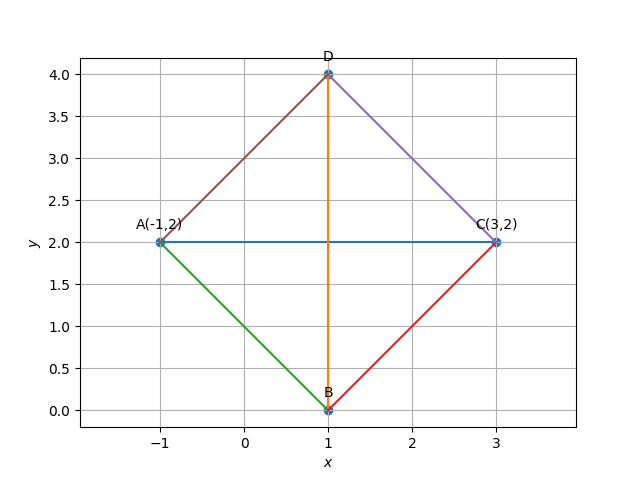
\includegraphics[width=\columnwidth]{chapters/10/7/4/4/figs/square}
	\end{center}
\caption{}
\label{fig:7/4/4/4Fig1}
\end{figure}

Shifting $\vec{A}$ to origin with reference to Fig. \ref{fig:7/4/4/4Fig2},
\begin{align}
\vec{A^{\prime}} =
\myvec{
0 \\
0\\
},
\vec{C^{\prime}} = \vec{C}-\vec{A} = 
\myvec{
4 \\
0\\
}
\end{align}

\begin{figure}[!h]
	\begin{center} 
	    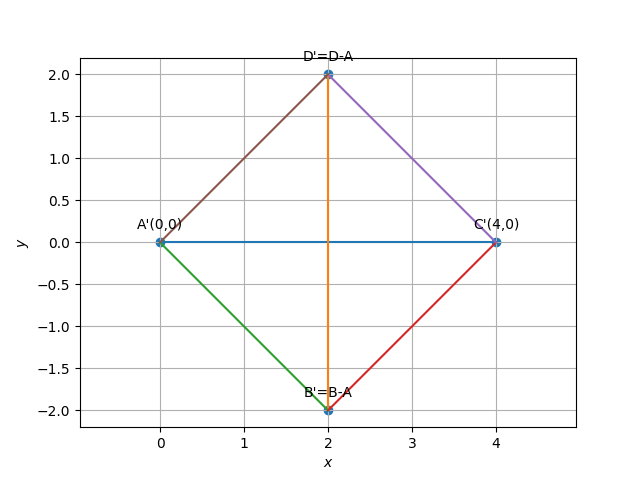
\includegraphics[width=\columnwidth]{chapters/10/7/4/4/figs/square1}
	\end{center}
\caption{}
\label{fig:7/4/4/4Fig2}
\end{figure}
\iffalse
In general,
the angle made by $AC$ with the x-axis is 
		\begin{align}
\beta = \theta + 45\degree
		\end{align}
\fi
Since
\begin{align}
\vec{C} - \vec{A} = \myvec{
4\\
0
} \equiv 
\myvec{
1\\
0
},
	\tan\theta&= \frac{0}{4} \implies 
\theta= 0\degree
\end{align}
		where
$\theta$ is the angle made by $AC$ with the x-axis.
Considering the rotation matrix 
\begin{align}
\vec{P} =
\myvec{
\cos\brak{\frac{\pi}{4}-\theta} & -\sin\brak{\frac{\pi}{4}-\theta} \\
\sin\brak{\frac{\pi}{4}-\theta} & \cos\brak{\frac{\pi}{4}-\theta} 
}
\end{align}
\iffalse
from Fig. \ref{fig:7/4/4/4Fig3},
\begin{align}
\vec{C^{\prime \prime}} = \vec{P}^\top (\vec{C}-\vec{A}) =
\myvec{
\frac{1}{\sqrt{2}} & -\frac{1}{\sqrt{2}} \\
\frac{1}{\sqrt{2}} & \frac{1}{\sqrt{2}}\\
}
\myvec{
4 \\
0\\
} = 
\myvec{
\frac{4}{\sqrt{2}} \\
\frac{4}{\sqrt{2}}\\
}
\end{align}
\begin{align}
\vec{B^{\prime \prime}} = \myvec{
 1&0\\
 0&0\\
}\vec{C^{\prime \prime}}=
\myvec{
 \frac{4}{\sqrt{2}}\\
 0\\
},
\vec{D^{\prime \prime}} = \myvec{
 0&0\\
 0&1\\
}\vec{C^{\prime \prime}}=
\myvec{
 0\\
 \frac{4}{\sqrt{2}}\\
} \text{ and }
\vec{A^{\prime \prime}} =
\myvec{
0 \\
0\\
}
\end{align}
\fi
\begin{figure}[!h]
	\begin{center} 
	    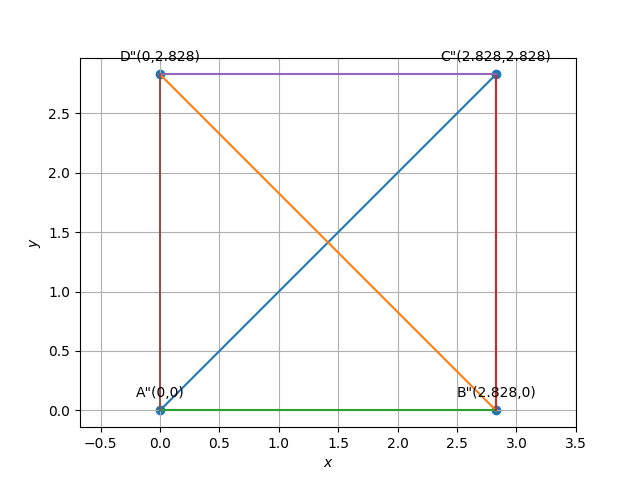
\includegraphics[width=\columnwidth]{chapters/10/7/4/4/figs/square2}
	\end{center}
\caption{}
\label{fig:7/4/4/4Fig3}
\end{figure}

\newpage
\iffalse
Again tranforming(rotating) the coordinates back to the original axis.

We know for anti-clockwise direction the rotation matrix is given as
\begin{align}
\vec{P} =
\myvec{
\cos\theta & -\sin\theta \\
\sin\theta & \cos\theta \\
}
\end{align}

Again we know that the angle is negative so the rotation will be in clockwise direction. So now the transformed(rotated) coordinates $\vec{B} \text{ and } \vec{D}$ are with refrence to 
\fi
from Figure 
%\ref{fig:7/4/4/4Fig4},
\ref{fig:7/4/4/4Fig3},
\begin{align}
	\vec{C^{\prime \prime}} &= \vec{P} (\vec{C}-\vec{A}) 
	\\
\label{eq:7/4/4/4bp}
	\vec{B^{\prime \prime}} &= \myvec{\vec{e}_1 & \vec{0}}\vec{C^{\prime \prime}}
	\\
\label{eq:7/4/4/4dp}
	\vec{D^{\prime \prime}} &= \myvec{ \vec{0} & \vec{e}_2}\vec{C^{\prime \prime}}
\end{align}
Now, 
\begin{align}
\label{eq:7/4/4/4b}
	\vec{B} = \vec{P}^{\top}\vec{B}^{\prime \prime}+\vec{A}
	\\
\label{eq:7/4/4/4d}
	\vec{D} = \vec{P}^{\top}\vec{D}^{\prime \prime}+\vec{A}
\end{align}
by reversing the process of translation and rotation.  Thus, 
from
\eqref{eq:7/4/4/4b}
\eqref{eq:7/4/4/4bp},
\eqref{eq:7/4/4/4d}
and
\eqref{eq:7/4/4/4dp}
\begin{align}
	\vec{B} = \vec{P}^{\top}\myvec{\vec{e}_1 & \vec{0}}\vec{P} (\vec{C}-\vec{A}) +\vec{A}
	\\
	\vec{D} = \vec{P}^{\top}\myvec{\vec{0} & \vec{e}_2  }\vec{P} (\vec{C}-\vec{A}) +\vec{A}
%	\vec{B} &= \brak{(\vec{C}-\vec{A})^{\top}\vec{P}^{\top} \vec{e}_1}\vec{P}^{\top}\vec{e}_1+\vec{A}
%	\\
%	\vec{D} &= \brak{(\vec{C}-\vec{A})^{\top}\vec{P}^{\top} \vec{e}_2}\vec{P}^{\top}\vec{e}_2+\vec{A}
\end{align}
yielding
		\begin{align}
\vec{B}=
\myvec{
1\\
0
},
\vec{D}
\myvec{
1\\
4
}.
		\end{align}
\iffalse
\begin{align}
\vec{B^{\prime}} &= \vec{P}\vec{B^{\prime \prime}} = \myvec{
\frac{1}{\sqrt{2}} & \frac{1}{\sqrt{2}} \\
-\frac{1}{\sqrt{2}} & \frac{1}{\sqrt{2}}\\
}
\myvec{
 \frac{4}{\sqrt{2}}\\
 0\\
} = 
\myvec{
2 \\
-2\\
}\\
\vec{D^{\prime}} &= \vec{P}\vec{D^{\prime \prime}} = \myvec{
\frac{1}{\sqrt{2}} & \frac{1}{\sqrt{2}} \\
-\frac{1}{\sqrt{2}} & \frac{1}{\sqrt{2}}\\
}
\myvec{
 0\\
 \frac{4}{\sqrt{2}}\\
} = 
\myvec{
2 \\
2 \\
}
\end{align}

\begin{figure}[!h]
	\begin{center} 
	    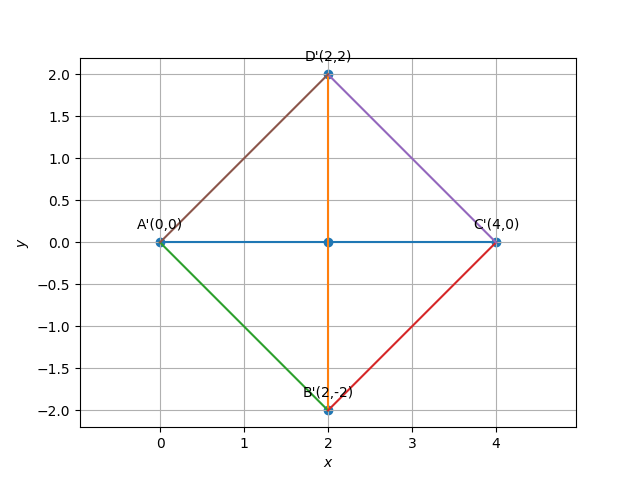
\includegraphics[width=\columnwidth]{chapters/10/7/4/4/figs/square3}
	\end{center}
\caption{}
\label{fig:7/4/4/4Fig4}
\end{figure}

Again transforming(shifting) the axis back to the original with refrence to Figure \ref{fig:7/4/4/4Fig5}
\begin{align}
\vec{B} &= \vec{B^{\prime}}+\vec{A} = \myvec{
2 \\
-2\\
}+\myvec{
-1 \\
2\\
} = 
\myvec{
1 \\
0\\
}\\
\vec{D} &= \vec{D^{\prime}}+\vec{A} = \myvec{
2 \\
2\\
}+\myvec{
-1 \\
2\\
} = 
\myvec{
1 \\
4 \\
}
\end{align}

Hence, the other two vertices are $\vec{B}(1,0) \text{ and } \vec{D}(1,4)$   

\begin{figure}[!h]
	\begin{center} 
	    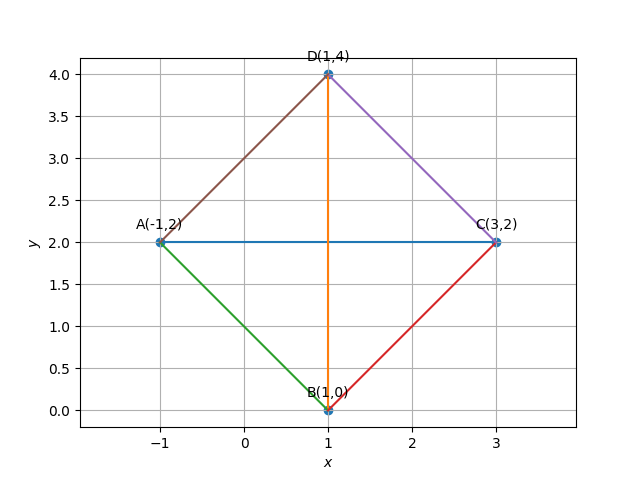
\includegraphics[width=\columnwidth]{chapters/10/7/4/4/figs/square4}
	\end{center}
\caption{}
\label{fig:7/4/4/4Fig5}
\end{figure}
which can also be expressed as
\begin{align}
\vec{B} &= \vec{A} + \vec{P}\myvec{
\vec{e_{1}}&\vec{0}\\
}
\vec{P}^\top \brak{\vec{C}-\vec{A}}\\
\vec{D} &= \vec{A} + \vec{P}\myvec{
\vec{0}&\vec{e_{2}}\\
}
\vec{P}^\top \brak{\vec{C}-\vec{A}}\\
\end{align}
where $\vec{P}$ is the rotation matrix and $\vec{A} \text{ and } \vec{C}$ are the position vectors of opposite vertices.

Derivation of the above formulas:

We know that after shifting the axis and rotating by the required angle any arbitrary square will be aligned with the x and y axis so that we can directly get the vectors $\vec{B} \text{ and } \vec{D}$ as follows
\begin{align}
\vec{C^{\prime\prime}} &= \vec{P}^\top \brak{\vec{C} - \vec{A}}\\
\vec{B^{\prime\prime}} &= \myvec{
\vec{e_{1}} & \vec{0}
}\vec{C^{\prime\prime}} = \myvec{
\vec{e_{1}} & \vec{0}
}\vec{P}^\top \brak{\vec{C} - \vec{A}}\\
\vec{B^{\prime}} &= \vec{P} \vec{B^{\prime\prime}}  = \vec{P}\myvec{
\vec{e_{1}} & \vec{0}
}\vec{P}^\top \brak{\vec{C} - \vec{A}}\\
\vec{B} &= \vec{A}+\vec{B^{\prime}}\\
 &= \vec{A} + \vec{P}\myvec{
\vec{e_{1}}&\vec{0}\\
}
\vec{P}^\top\brak{\vec{C}-\vec{A}}
\end{align}

Similarly for D it can be derived as
\begin{align}
\vec{C^{\prime\prime}} &= \vec{P}^\top \brak{\vec{C} - \vec{A}}\\
\vec{D^{\prime\prime}} &= \myvec{
\vec{0} & \vec{e_{2}}
}\vec{C^{\prime\prime}} = \myvec{
\vec{0} & \vec{e_{2}}
}\vec{P}^\top \brak{\vec{C} - \vec{A}}\\
\vec{D^{\prime}} &= \vec{P} \vec{D^{\prime\prime}} = \vec{P} \myvec{
\vec{0} & \vec{e_{2}}
}\vec{P}^\top \brak{\vec{C} - \vec{A}}\\
\vec{D} &= \vec{A}+\vec{D^{\prime}}\\
 &= \vec{A} + \vec{P}\myvec{
\vec{0}&\vec{e_{2}}\\
}
\vec{P}^\top\brak{\vec{C}-\vec{A}}
\end{align}


Verification of the above formula for the given question

\begin{align}
\vec{B} &= \myvec{
-1\\
2\\
}+\myvec{
\frac{1}{\sqrt{2}} & \frac{1}{\sqrt{2}} \\
-\frac{1}{\sqrt{2}} & \frac{1}{\sqrt{2}}\\
}\myvec{
 1&0\\
 0&0\\
}\myvec{
\frac{1}{\sqrt{2}} & -\frac{1}{\sqrt{2}} \\
\frac{1}{\sqrt{2}} & \frac{1}{\sqrt{2}}\\
}\myvec{
4\\
0\\
}\\
 &= \myvec{
-1\\
2\\
}+\myvec{
\frac{1}{\sqrt{2}} & \frac{1}{\sqrt{2}} \\
-\frac{1}{\sqrt{2}} & \frac{1}{\sqrt{2}}\\
}\myvec{
 1&0\\
 0&0\\
}\myvec{
\frac{4}{\sqrt{2}}\\
\frac{4}{\sqrt{2}}\\
}\\
 &= \myvec{
-1\\
2\\
}+\myvec{
\frac{1}{\sqrt{2}} & \frac{1}{\sqrt{2}} \\
-\frac{1}{\sqrt{2}} & \frac{1}{\sqrt{2}}\\
}\myvec{
\frac{4}{\sqrt{2}}\\
0\\
}\\
 &= \myvec{
-1\\
2\\
}+\myvec{
2\\
-2\\
}\\
 &= \myvec{
1\\
0\\
}\\
\vec{D} &= \myvec{
-1\\
2\\
}+\myvec{
\frac{1}{\sqrt{2}} & \frac{1}{\sqrt{2}} \\
-\frac{1}{\sqrt{2}} & \frac{1}{\sqrt{2}}\\
}\myvec{
 0&0\\
 0&1\\
}\myvec{
\frac{1}{\sqrt{2}} & -\frac{1}{\sqrt{2}} \\
\frac{1}{\sqrt{2}} & \frac{1}{\sqrt{2}}\\
}\myvec{
4\\
0\\
}\\
 &= \myvec{
-1\\
2\\
}+\myvec{
\frac{1}{\sqrt{2}} & \frac{1}{\sqrt{2}} \\
-\frac{1}{\sqrt{2}} & \frac{1}{\sqrt{2}}\\
}\myvec{
 0&0\\
 0&1\\
}\myvec{
\frac{4}{\sqrt{2}}\\
\frac{4}{\sqrt{2}}\\
}\\
 &= \myvec{
-1\\
2\\
}+\myvec{
\frac{1}{\sqrt{2}} & \frac{1}{\sqrt{2}} \\
-\frac{1}{\sqrt{2}} & \frac{1}{\sqrt{2}}\\
}\myvec{
0\\
\frac{4}{\sqrt{2}}\\
}\\
 &= \myvec{
-1\\
2\\
}+\myvec{
2\\
2\\
}\\
 &= \myvec{
1\\
4\\
}
\end{align}
\fi








\item The base of an equilateral triangle with side $2a$ lies along the y-axis such that the mid-point of the base is at the origin. Find vertices of the triangle.
\label{chapters/11/10/1/2}
\iffalse
\documentclass[journal,12pt,twocolumn]{IEEEtran}
\usepackage{graphicx}
\usepackage{listings}
\usepackage[utf8]{inputenc}
\usepackage{caption}
\usepackage{hyperref}
\usepackage[cmex10]{amsmath}
\usepackage{array}
\usepackage{gensymb}
\usepackage{booktabs}
\usepackage{etoolbox}
\patchcmd{\section}{\centering}{}{}{}
\providecommand{\norm}[1]{\left\lVert#1\right\rVert}
\providecommand{\abs}[1]{\left\vert#1\right\vert}
\let\vec\mathbf
\newcommand{\myvec}[1]{\ensuremath{\begin{pmatrix}#1\end{pmatrix}}}
\newcommand{\mydet}[1]{\ensuremath{\begin{vmatrix}#1\end{vmatrix}}}
\providecommand{\brak}[1]{\ensuremath{\left(#1\right)}}
\makeatletter
\newcommand\xleftrightarrow[2][]{%
  \ext@arrow 9999{\longleftrightarrowfill@}{#1}{#2}}
\newcommand\longleftrightarrowfill@{%
  \arrowfill@\leftarrow\relbar\rightarrow}
\makeatother
\title{Matrix Problems \textbf{\\Straight Lines }}
\author{Manoj Chavva} 

\begin{document}
\maketitle



\section{Problem Statement}

\noindent 
\fi
	\begin{figure}[!ht]
		\centering
 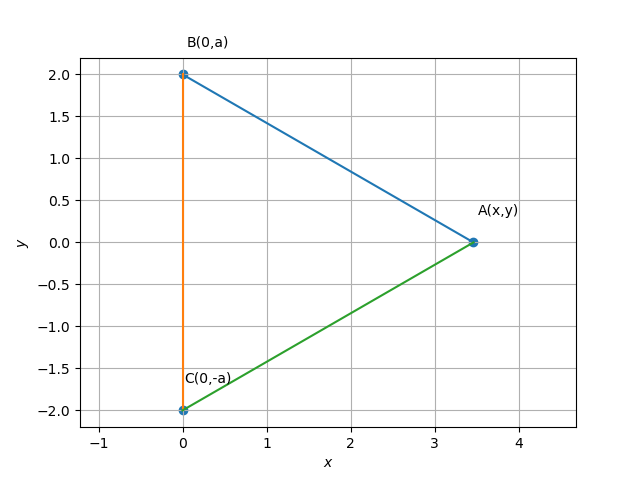
\includegraphics[width=\columnwidth]{chapters/11/10/1/2/figs/triangle.png}
		\caption{}
		\label{fig:11/10/1/2}
  	\end{figure}
	\\
	\solution Let the base be $BC$.  From the given information, 
\begin{align}
	\vec{B} = a\vec{e}_2,
	\vec{C} = -a\vec{e}_2
\end{align}
Since $\vec{A}$ lies on the $x$-axis, 
\begin{align}
	\vec{A} = k\vec{e}_1
\end{align}
and 
\begin{align}
	\norm{\vec{A}-\vec{C}}^2 &= \brak{2a}^2
	\\
	\implies \norm{\vec{A}}^2+\norm{\vec{C}}^2 - 2 \vec{A}^{\top}\vec{C} &= 4a^2
	\\
	\implies k^2 +a^2 &= 4a^2
	\\
	\text{or, } k = \pm a\sqrt{3}
\end{align}
Thus, 
\begin{align}
	\vec{A} = \pm \sqrt{3}a\vec{e}_1
\end{align}
		Fig. \ref{fig:11/10/1/2}
		is plotted for $a = 2$.

\iffalse

\begin{figure}[h]
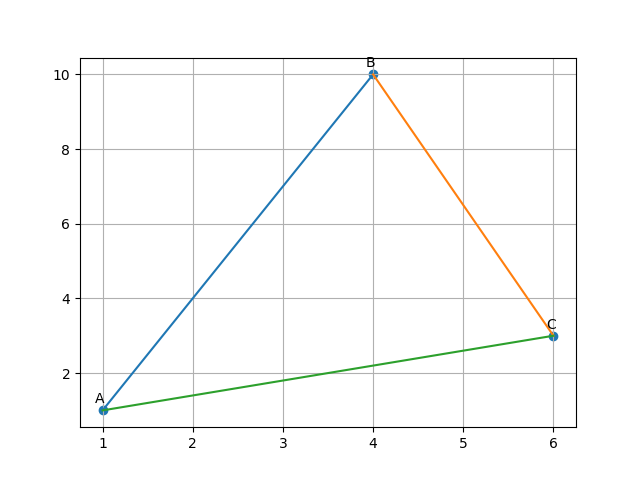
\includegraphics[width=1\columnwidth]{triangle.png}
\caption{Equilateral Triangle ABC}
\label{fig:triangle}
\end{figure}

\section{Construction}
B and C are the inputs.
\begin{table}[h]
\centering
\large
\begin{tabular}{|l|l|l|}
\hline
\textbf{Symbol} & \textbf{Value} & \textbf{Description} \\ \hline
B               & \myvec{0 \\ 2}         & Vertex B             \\ \hline
C               & \myvec{0 \\ -2}        & Vertex C             \\ \hline
A               & \myvec{x \\ y}          & Vertex A             \\ \hline
A1              & \myvec{x1 \\ y1}       & Vertex A             \\ \hline
\end{tabular}
\end{table}

\section{Solution}
\noindent Given the base with 2a is lies on the y-axis with the mid-point of the base is at origin. The vertices of the two points on y-axis will be

\begin{equation}
\vec{B}=\begin{pmatrix} 
0\\
a
\end{pmatrix}, {
\vec{C}=\begin{pmatrix} 
0\\
-a
\end{pmatrix} }
\end{equation}
\noindent Given $\Delta$ABC is an equilateral triangle i.e 
\begin{equation}
 \norm{\vec{A}-\vec{B}}= \norm{\vec{B}-\vec{C}}= \norm{\vec{C}-\vec{A}} =2a
\end{equation}

%\noindent As AB = AC, triangle is isoceles and by properties of isoceles triangle, altitude is perpendicular bisector of base.\\
%
%\noindent Therefore $\angle$AOC = $\angle$AOB = $90^0$ and $\norm{\vec{O}-\vec{B}}= \norm{\vec{O}-\vec{C}}= a$ \\
%
%\noindent By Cosine laws,
%\begin{equation}
%\cos\vec{B} = \cos\vec{C} = a* \frac{1}{2a} = \frac{1}{2}
%\end{equation}
%\begin{equation}
%\angle B = \angle C = \arccos\frac{1}{2} = 60^0
%\end{equation}
% \begin{equation}
% \angle A = 180^0 -(60^0 * 2) = 60^0
%  \end{equation}
%\noindent Therefore, the equilaterial triangle have all internal angles eaqual to  $60^0$ 

\noindent Consider, two sides of equilateral triangle be $\vec{A}$ and $\vec{B}$ then the third side will be $ \vec{A} -\vec{B}$ 
%Hence,
%\begin{equation}
%\norm{\vec{a}-\vec{b}}^2 = l
%\end{equation}
%\begin{equation}
%\brak{\vec{a}-\vec{b}}^{\top} \brak{\vec{a}-\vec{b}} = l^2
%\end{equation}
%\begin{equation}
%l^2 = 2 \vec{a}^{\top} \cdot \vec{b}
%\end{equation}
%\begin{equation}
%l^2 = 2 \norm{\vec{a}}\norm{\vec{b}} \cos\theta
%\end{equation}
%\begin{equation}
%\theta = \arccos\frac{1}{2} = 60^0
\begin{equation}
\norm{\vec{A}}=\norm{\vec{B}}=\norm{\vec{A-B}}\\
\end{equation}
\begin{equation}
\norm{\vec{A}}^2=\norm{\vec{B}}^2=\norm{\vec{A-B}}^2\\
\end{equation}
\begin{equation}
\norm{\vec{A}}^2+\norm{\vec{B}}^2-2\vec{A}^T\vec{B}=\norm{\vec{A}}^2=\norm{\vec{B}}^2\\
\end{equation}
\begin{equation}
\frac{\vec{A}^T\vec{B}}{\norm{\vec{A}}^2}=\frac{\vec{A}^T\vec{B}}{\norm{\vec{B}^2}}=\frac{1}{2}
\end{equation}
%$\triangle$OAB is a equilateral triangle\\

\noindent Therefore, the  triangle have all internal angles eaqual to  $60^0$

The angle between two vectors is given by 
  \begin{align}
    \label{eq:angle2d}
    \theta = \cos^{-1}\frac{\vec{A}^{\top} \vec{B}}{\norm{A}\norm{B}}
  \end{align}

 \begin{equation}  
  \brak{\vec{x}-\vec{B}}^{\top} \brak{\vec{x}-\vec{C}}= \norm{\vec{x}-\vec{B}} \cdot \norm{\vec{x}-\vec{C}} \cdot \cos\theta 
 \end{equation}

 \begin{equation}  
\brak{\vec{x}^\top \cdot \vec{x}} - \brak{\vec{x}^\top \cdot \vec{C}} - \brak{\vec{B}^\top \cdot \vec{x}} - \brak{\vec{B}^\top \cdot \vec{C}} = 2a \cdot 2a \cos 60^0   
 \end{equation}

 \begin{equation}  
\norm{\vec{x}}^2 - \vec{x}^\top\brak{\vec{B}+\vec{C}} - \vec{B}^\top \cdot \vec{C} = 2a \cdot 2a \cdot \frac{1}{2}
 \end{equation}

  \begin{equation}  
\norm{\vec{x}}^2 - \vec{x}^\top\brak{0} -\myvec{0 \\ a} \myvec{0 & -a}  = 4a^2
 \end{equation}

\begin{equation}
\norm{\vec{x}}^2 + a^2 = 4a^2
\end{equation}

\begin{equation}
\norm{\vec{x}}^2 = 3a^2
\label{eq-1}
\end{equation}
Considering, the line equation of $\vec{AB}$

\begin{equation}
\norm{\vec{x}-\vec{B}}^2 = 4a^2
\end{equation}

\begin{equation}
\brak{\vec{x} -\vec{B}}^{\top} \cdot \brak{\vec{x}-\vec{B}} = 4a^2
\end{equation}

\begin{equation}
\norm{\vec{x}}^2-2\cdot \vec{x}^\top \vec{B} + \norm{\vec{B}}^2 = 4a^2
\end{equation}

\begin{equation}
3a^2 - 2\cdot \vec{x}^\top \vec{B} + a^2 = 4a^2
\end{equation}

\begin{equation}
\vec{x}^\top \vec{B} = 0
\end{equation}
\noindent Since we can write, \begin{equation}
\vec{B} = a \cdot \vec{e}_2
\end{equation}

\begin{equation}
\vec{x}^\top \cdot a \cdot \vec{e}_2 = 0
\end{equation}

\begin{equation}
\vec{x}^\top \cdot \vec{e}_2 = 0
\end{equation}

\begin{equation}
\vec{x} = \lambda \vec{e}_1
\end{equation}

\noindent From this its clearly concluded that third vertex will lie on x-axis. 
\noindent From the equation \eqref{eq-1} 
\begin{equation}
\vec{x} = \sqrt{3}{a}
\end{equation}


\noindent Hence,the coordinates of the vertices of triangle are 
  \begin{equation*}
\vec{A} = 
   \begin{pmatrix}
   \pm\sqrt{3}a \\ 0
 \end{pmatrix}
 \end{equation*}

\begin{equation}
\vec{B}=\begin{pmatrix} 
0\\
a
\end{pmatrix}, {
\vec{C}=\begin{pmatrix} 
0\\
-a
\end{pmatrix} }
\end{equation}



\begin{table}[h]
\large
\begin{tabular}{lll}
\multicolumn{3}{l}{Get Python Code for image from}                                                 \\ \hline
\multicolumn{3}{|l|}{\url{https://github.com/ManojChavva/FWC/blob/main/Matrix/line/code-py/triangle.py}} \\ 
 \hline
\multicolumn{3}{l}{Get LaTex code from}                                                            \\ \hline
\multicolumn{3}{|l|}{\url{https://github.com/ManojChavva/FWC/blob/main/Matrix/line/line.tex}}            \\ \hline
\end{tabular}
\end{table}

\end{document}

\fi

\item The value of the expression $\abs{\vec{a}\times\vec{b}}$+ $({\vec{a}.\vec{b}})$ is \rule{1cm}{0.15mm}.
\item If $\abs{\vec{a}\times\vec{b}}^2$ + $\abs{\vec{a}.\vec{b}}^2$=144 $\text{and}$  $\abs{\vec{a}}$=4, then $\abs{\vec{b}}$ is equal to \rule{1cm}{0.15mm}.
\item If the directions cosines of a line are $(k,k,k)$ then
\begin{enumerate}
	\item $k>0$
	\item $0<k<1$
	\item $k=1$ 
	\item $k=\dfrac{1}{\sqrt{3}}$ or $-\dfrac{1}{\sqrt{3}}$
\end{enumerate}
\item  Find the position vector of a point A in space such that $\overrightarrow{OA}$ is inclined at $60 \degree$ to OX and at $45 \degree$ to OY and $\abs{\overrightarrow{OA}} =10$ units.
\item If $(-4,3)\text{ and }(4,3)$ are two vertices of an equilateral triangle. Find the coordinates of the third vertex, given that the origin lies in the interior of the triangle. 
\item $\vec{A} (6,1),\vec{B}(8,2) \text{ and } \vec{C}(9,4)$ are three vertices of a parallelogram ABCD. If $\vec{C}$ is the midpoint of DC find the area of $\triangle ADE$
\item If the points  $\vec{A}(1,-2), \vec{B}(2,3) , \vec{C}(a,2)\text{ and }\vec{D} (-4-3)$ form parallelogram, find the value of $a$ and height of the parallelogram taking AB as base.
\item Ayush starts walking from his house to office. Instead of going to the office directly, he goes to a bank first, from there to his daughter school and then reaches the office what is the extra distance travelled by Ayush in reaching his office? (Assume that all distanes covered are in straight lines). If the house is situated at $(2,4)$, bank at $(5,8)$, school at $(13,14)$ and office at $(13,26)$ and coordinates are in km.
\item Find the angle between the lines whose direction cosines are given by the equations $l+m+n=0$, $l^2+m^2-n^2=0$.
\item If a variable line in two adjacent positions has directions cosines $l, m, n$ and $l+\delta l, m+\delta m, n+\delta n$, show that the small angle $\delta\theta$ between the two positions is given by 
\begin{align}
	\delta\theta^2=\delta l^2+\delta m^2+\delta n^2
\end{align}
\item The vector $\vec{a}+\vec{b}$ bisects the angle between the non-collinear vectors $\vec{a}$ $\text{ and }$ $\vec{b}$ if \rule{1cm}{0.15mm}.
\item If $\vec{a}$ $\text{ and }$ $\vec{b}$ are adjacent sides of a rhombus, then $\vec{a}\cdot \vec{b}$=0.
\item Let $\vec{a}$ and $\vec{b}$ be two unit vectors and $\theta$ the angle between them. Then $\vec{a}+\vec{b}$ is a unit vector if
	\begin{enumerate}
			\itemsep2pt
		\item $\theta = \frac{\pi}{4}$
		\item $\theta = \frac{\pi}{3}$
		\item $\theta = \frac{\pi}{2}$
		\item $\theta = \frac{2\pi}{3}$
			\end{enumerate}
\solution
Given,
\begin{align}
	\norm{\vec{a}}=\norm{\vec{b}}=1\label{eq:12/10/5/17/1}
	\\
	\norm{\vec{a}+\vec{b}}=1\label{eq:12/10/5/17/2}
\end{align}
Squaring both sides of \eqref{eq:12/10/5/17/2}  , we get
\begin{align}
	\norm{\vec{a}+\vec{b}}^2=1^2
\\	
	\implies \norm{\vec{a}}^2 + \norm{\vec{b}}^2 + 2\vec{a}^{\top}\vec{b} = 1\label{eq:12/10/5/17/3}	
\end{align}
Substituting \eqref{eq:12/10/5/17/1} in \eqref{eq:12/10/5/17/3}, we get
\\
\begin{align}
	\implies 1+1+2(\norm{\vec{a}}\norm{\vec{b}}\cos{\theta})=1
	\\
	\implies 2+2(\norm{\vec{a}}\norm{\vec{b}}\cos{\theta})=1
        \\
	\implies 2(\norm{\vec{a}}\norm{\vec{b}}\cos{\theta})=-1
	\\
	\implies (\norm{\vec{a}}\norm{\vec{b}}\cos{\theta})=\frac{-1}{2}\label{eq:12/10/5/17/4}
\end{align}
Subtituting \eqref{eq:12/10/5/17/1} in \eqref{eq:12/10/5/17/4}, we get
\begin{align}
	\implies \cos{\theta}=\frac{-1}{2}
	\\
	\implies \theta=\frac{2\pi}{3}
\end{align}

\item Show that the tangent of an angle between the lines 
\begin{align}
	\frac{x}{a}+\frac{y}{b}&=1 \text{ and }
	\\
	\frac{x}{a}-\frac{y}{b}&=1 
\end{align}
is $\frac{2ab}{a^2-b^2}$.
\item Find $\abs{\overrightarrow {x}}$, if for a unit vector $\overrightarrow {a}, (\overrightarrow {x}-\overrightarrow {a})\cdot (\overrightarrow {x}+\overrightarrow {a}$)=12.
	\\
\solution 
		From the given information,
\begin{align}
  \label{eq:12/10/3/9det2f}
  \brak{\vec{x}-\vec{a}}^\top\brak{\vec{x}+\vec{a}} &= 12 \\
  \implies \norm{\vec{x}}^{2} - \norm{\vec{a}}^{2} &= 12 \\
\implies   
	\norm{\vec{x}} &= \sqrt{13}
\end{align}

\item Find $\abs{\overrightarrow {a}}$ and $\abs{\overrightarrow {b}}$, if ($\overrightarrow {a}+\overrightarrow {b})\cdot (\overrightarrow {a}-\overrightarrow {b})=8$ and $\abs{\overrightarrow {a}}=8\abs{\overrightarrow {b}}$.
	\\
	\solution
		\begin{align}
\because \brak{\vec{a}+\vec{b}}^\top\brak{\vec{a}-\vec{b}}=8,
\norm{\vec{a}} &= 8\norm{\vec{b}},\\
\norm{\vec{a}}^2-\norm{\vec{b}}^2&=8\\
\implies\norm{8\vec{b}}^2-\norm{\vec{b}}^2&=8\\
\implies \norm{\vec{b}}&=\frac{2\sqrt{2}}{3\sqrt{7}}
\end{align}
Thus, 
\begin{align}
\norm{\vec{a}}&=8\norm{\vec{b}}
=\frac{16\sqrt{2}}{3\sqrt{7}}
\end{align}

\item Find the magnitude of two vectors $\overrightarrow {a}$ and $\overrightarrow {b}$, having the same magnitude and such that the angle between them is $60\degree$ and their scalar product is $\frac{1}{2}$.
	\\
	\solution
		Given 
\begin{align}
	\norm{\vec{a}}= \norm{\vec{b}}, {\cos\theta} = \frac{1}{2}, 
	\vec{a}^{\top}{\vec{b}} = \frac{1}{2},  \\
\implies 
	\frac{1}{2} = \frac{\frac{1}{2}}{\norm{\vec{a}}^2}
\implies \norm{\vec{a}}
= \norm{\vec{b}}=1
\end{align}
by using  the definition of the scalar product.

\item Show that $\abs {\overrightarrow {a}}\overrightarrow {b}+\abs{\overrightarrow {b}}\overrightarrow {a}$ is perpendicular to $\abs{\overrightarrow {a}} \overrightarrow {b}-\abs{\overrightarrow {b}} \overrightarrow {a}$, for any two nonzero vectors $\overrightarrow {a}$ and $\overrightarrow {b}$.
	\\
	\solution
		\begin{align}
\norm{\vec{a}}\vec{b}+\norm{\vec{b}}\vec{a}
=
	\norm{\vec{a}}\norm{\vec{b}}\brak{\frac{\vec{b}}{\norm{\vec{b}}}+\frac{\vec{a}}{\norm{\vec{a}}}}
	\\
\norm{\vec{a}}\vec{b}-\norm{\vec{b}}\vec{a}
=
	\norm{\vec{a}}\norm{\vec{b}}\brak{\frac{\vec{b}}{\norm{\vec{b}}}-\frac{\vec{a}}{\norm{\vec{a}}}}
	\\
	\implies 
	\brak{\norm{\vec{a}}\vec{b}+\norm{\vec{b}}\vec{a}}^{\top} \brak{\norm{\vec{a}}\vec{b}-\norm{\vec{b}}\vec{a}} = 0
\end{align}
	from \eqref{eq:12/10/3/11/unit}.

\item If $\overrightarrow {a},\overrightarrow {b},\overrightarrow {c}$ are unit vectors such that $\overrightarrow {a}+\overrightarrow {b}+\overrightarrow {c}=\overrightarrow {0}$, find the value of $\overrightarrow {a}.\overrightarrow {b}+\overrightarrow {b}.\overrightarrow {c}+\overrightarrow {c}.\overrightarrow {a}$.
	\\
	\solution
		\begin{align}
	\norm{{\vec{a}}+{\vec{b}}+{\vec{c}}}^2=0
	\nonumber \\
	\implies{\norm{\vec{a}}}^2+{\norm{\vec{b}}}^2+{\norm{\vec{c}}}^2+2({{\vec{a}^\top}{\vec{b}}+{\vec{b}^\top}{\vec{c}}+{\vec{c}^\top}{\vec{a}}})=0
	\nonumber \\
	\implies3+2({{\vec{a}^\top}{\vec{b}}+{\vec{b}^\top}{\vec{c}}+{\vec{c}^\top}{\vec{a}}})=0\nonumber \\
	\implies{\vec{a}^\top}{\vec{b}}+{\vec{b}^\top}{\vec{c}}+{\vec{c}^\top}\vec{a}=-\frac{3}{2}
\end{align}

\item If either vector $\overrightarrow {a}=0$ or $\overrightarrow {b}=0$, then $\overrightarrow {a}.\overrightarrow {b}$=0. But the converse need not be true. Justify your answer with an example.
	\\
	\solution
		\begin{align}
	\vec{a}=\myvec{1\\1},\,
\vec{b}=\myvec{1\\-1}\\
\implies \vec{a} ^\top \vec{b} =  0 
\end{align}



\item Prove that $(\vec{a}+\vec{b})\cdot(\vec{a}+\vec{b})=|{\vec{a}}|^2+|{\vec{b}}|^2$, if and only if $\vec{a}, \vec{b}$ are perpendicular, given $\vec{a}\neq\vec{0}, \vec{b}\neq\vec{0}$.\\
	\solution
			\begin{align}
\because 		\brak{\vec{a}+\vec{b}}^{\top}\brak{\vec{a}+\vec{b}} 
		= \norm{\vec{a}}^2+\norm{\vec{b}}^2,
		\\
		 \norm{\vec{a}}^2+\norm{\vec{b}}^2+2\vec{a}^{\top}\vec{b}
		= \norm{\vec{a}}^2+\norm{\vec{b}}^2
		\\
		\implies 
		\vec{a}^{\top}\vec{b} = 0 
	\end{align}


	\item  If $l_1, m_1,n_1 \text{ and } l_2,m_2,n_2$ are the direction cosines of two mutually perpendicular lines, show that the direction cosines of the line perpendicular to both these are  $m_1n_2-m_2n_1,n_1l_2-n_2l_1,l_1m_2-l_2m_1$.
\\
    \solution
		\begin{align}
\vec{P} 
	=\myvec{
l_1&l_2&m_1n_2-m_2n_1\\
        m_1&m_2&n_1l_2-n_2l_1\\
        n_1&n_2&l_1m_2-l_2m_1
}
	\end{align}
	satisfies 
\eqref{eq:12/10/3/5/inner}.
	Hence, the three vectors are mutually perpendicular.

    \item If $ \vec{A},\vec{B},\vec{C} $ are mutually perpendicular vectors of equal magnitudes,show that the  $ \vec{A}+\vec{B}+\vec{C} $ is equally inclined to $ \vec{A},\vec{B}  \text{ and }  \vec{C} $.
\item Projection vector of $\vec{a}$ on $\vec{b}$ is
	\begin{enumerate}
\item $\left(\frac{\vec{a}\cdot\vec{b}}{\abs{\vec{b}}^2}\right)$
\item $\frac{\vec{a}\cdot\vec{b}}{\abs{\vec{b}}}$
\item $\frac{\vec{a}\cdot\vec{b}}{\abs{\vec{a}}}$
\item $\left(\frac{\vec{a}\cdot\vec{b}}{\abs{\vec{a}}^2}\right)$
\end{enumerate}
\item If $\vec{a}$ is  any non-zero vector, then $(\vec{a}\cdot \hat{i})\hat{i}$+$(\vec{a}\cdot \hat{j})\hat{j}$+$(\vec{a}\cdot \hat{k})$ $\hat{k}$ equals \rule{1cm}{0.15mm}.
\item If $\vec{a}$, $\vec{b}$, $\vec{c}$ are unit vectors such that $\vec{a}$+$\vec{b}$+$\vec{c}$=0, then the value of $\vec{a} \cdot \vec{b}+\vec{b} \cdot \vec{c}+\vec{c} \cdot \vec{a}$ is
	\begin{enumerate}
\item 1
\item 3
\item $\frac{-3}{2}$
\item None of these
\end{enumerate}
\item If $\vec{a},\vec{b},\vec{c}$ are the three vectors such that $\vec{a}+\vec{b}+\vec{c}=0$ $\text{ and }$ $|\vec{a}|=2$, $|\vec{b}|$=3, $|\vec{c}|$=5, the value of $\vec{a} \cdot \vec{b}+\vec{b} \cdot \vec{c}+\vec{c} \cdot \vec{a}$ is
	\begin{enumerate}
\item 0
\item 1	
\item -19
\item 38
\end{enumerate}
\item If $\vec{r}\cdot\vec{a}=0, \vec{r}\cdot\vec{b}=0$ and $\vec{r}\cdot\vec{c}=0$ for some non-zero vector $\vec{r}$, then the value of $\vec{a}\cdot(\vec{b}\times\vec{c})$ is \rule{1cm}{0.15mm}.
\item If $\abs{\vec{a}+\vec{b}}$ = $\abs{\vec{a}-\vec{b}}$, then the vectors $\vec{a}$ $\text {and}$ $\vec{b}$ are orthogonal.
\item Prove that the lines $x=py+q , z=ry+s \text{ and } x=p^{\prime}y+q^{\prime}, z=r^{\prime}y+s^{\prime} $ are perpendicular if $pp^{\prime}+rr^{\prime}+1=0$.
\item Show that the straight lines whose direction cosines are given by $2l+2m-n=0$ and $mn+nl+lm=0$ are at right angles.
\item If $l_1, m_1, n_1;l_2, m_2, n_2;l_3, m_3, n_3$ are the direction cosines of the three mutually perpendcular lines, prove that the line whose direction cosines are propotional to $l_1+l_2+l_3 , m_1+m_2,m_3, n_1+n_2+n_3$ make angles with them.
\item
Find the angle between the lines whose direction ratios are $a,b,c$ and $b-c,c-a,a-b$.
\\
\solution
    \begin{align}
\because \myvec{a&b&c}\myvec{b-c\\c-a\\a-b} = 0,
   \theta=\frac{\pi}{2}
    \end{align}

\end{enumerate}
